% Capítulo 2
\chapter{Arash}

\abrv[ARASH -- \textit{Anthropomorphic Robot Augmented with Sense of Human}, em livre tradução Robô Antropomórfico Aumentado com Sentido de Ser Humano]{ARASH}(\textit{Anthropomorphic Robot Augmented with Sense of Human}, em português Robô Antropomórfico Aumentado com Sentido de Ser Humano), além de um herói arqueiro da mitologia iraniana, é um robô de 7,5 Kg e 1 metro de altura. Possuindo 20 graus de liberdade (ou \abrv[DOF -- Do inglês \textit{Degrees Of Freedom}, ou graus de liberdade]{DOF}, do inglês \textit{degrees of freedom}), ele tenta imitar a configuração humana, tanto em suas juntas quanto em suas proporções. Em suas juntas, Arash possui motores MX-28, MX-64 e MX-106 (da Robotis Co), dependendo da carga suportada. Como controlador principal, um computador \textit{mini-box} é utilizado em conjunto com uma placa microcontroladora \textit{OpenCM9.04} que serve de interface entre o controlador principal e os motores \cite{autdp2016}.

\subsection{Graus de Liberdade e Atuadores}
\label{subsec:architecture:Atuators}

\todo{Adicionar um parágrafo introdutório.}
PARAGRAFO INTRODUTÓRIO.

Tão importante quanto a configuração das juntas é a orientação dos atuadores para que os cálculos funcionem como o esperado.

\begin{figure}[htb]
	\centering
	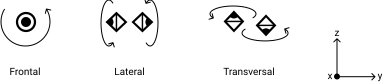
\includegraphics[scale=1]{imagens/svg/actuators-orientation}
	\caption{Orientação dos movimentos dos atuadores}
	\label{fig:ActuatorsOrientation}
\end{figure}

A figura~\ref{fig:ActuatorsOrientation} exibe as possíveis orientações dos atuadores que são referenciadas ao longo do trabalho como frontal, lateral e transversal.

Atuadores com orientação frontal -- ou simplesmente, atuadores frontais -- propiciam rotação orientada pelo eixo $X$, que está aponta para o leitor (para fora do papel). Esse tipo de rotação também é referida como \textit{roll}.

Atuadores laterais apontam para direita ou esquerda. Eles apresentam rotação com base no eixo $Y$ (plano $XZ$), também conhecida como rotação \textit{pitch}. Analogamente, atuadores transversais apontam para cima ou baixo, com base no eixo $Z$ (plano $XY$), com movimento de rotação conhecido como \textit{yaw}.

Na figura~\ref{fig:architecture:arash:actuators_orientations}, observa-se o esquema de orientação dos atuadores aplicada no diagrama das juntas de Arash. Ainda na mesma figura, os ``triângulos pretos preenchidos'' representam apenas o fim de uma cadeia de atuadores. Assim, estes símbolos representam as mãos, que não possuem atuadores, e a ponta da cabeça, onde encontra-se a câmera. 

Estas orientações são importantes durante os cálculos dos ângulos enviados às juntas. Já que a inconsistência do modelo matemático e o robô físico causa inversão de movimentos durante a caminhada, causando reações inesperadas e possíveis danos.

Em Arash, todos os atuadores utilizados são produzidos pela Robotics.Co. Porém, devido a variação de carga nas diversas juntas, foram utilizados diferentes  modelos da série MX. Esta decisão de projeto diminui bastante o custo final do robô.

\begin{figure}[htb]
	\centering
	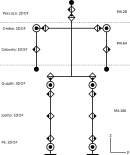
\includegraphics[scale=1]{imagens/svg/arash-schematics}
	\caption{Diagrama de orientação dos atuadores de Arash}
	\label{fig:architecture:arash:actuators_orientations}
\end{figure}

No pescoço, onde a carga é bem leve, ``MX-28'' são suficientes. Dois atuadores, um na posição transversal (o atuador mais baixo) que fornece o movimento panorâmico a cabeça e outro na posição horizontal, fornecendo o movimento de inclinação vertical da cabeça.

Nos braços, que podem sofrer uma carga maior, atuadores ``MX-64'' são utilizados. Isso é importante já que existem modalidades de competições, como o levantamento de peso, que testam a capacidade do carregamento de cargas.

Para as pernas, foram utilizados atuadores ``MX-106'' que são mais poderosos que os anteriores. Entretanto, na fase de projeto, simulações mostraram que durante o movimento de levantar-se do chão (em caso da recuperação de uma possível queda), o torque nas juntas do joelho era levado ao máximo suportado pelo ``MX-106'', podendo assim levar este motor à falha. Desta forma, 2 atuadores sincronizados passaram a formar esta junta, afim de compartilhar a carga sofrida entre dois motores. Esta junta dupla não oferece nenhum impacto na implementação, já que os motores da série ``MX-106'' oferecem a capacidade de serem ligados e sincronizados via \textit{hardware}. Assim, a nível de software controla-se apenas 1 único atuador. Desta forma, apesar das 20 DOF, Arash possui 22 motores.

\begin{guide}
	Falar sobre as tecnologias atuais de \textit{walking gait}.
\end{guide}

\begin{guide}
	Falar sobre a abordagem tomada para este trabalho.
\end{guide}

Este é o primeiro capítulo da parte central do trabalho, isto é, o desenvolvimento, a parte mais extensa de todo o trabalho. Geralmente o desenvolvimento é dividido em capítulos, cada um com subseções e subseções, cujo tamanho e número de divisões variam em função da natureza do conteúdo do trabalho.

Em geral, a parte de desenvolvimento é subdividida em quatro subpartes:

\begin{itemize}
   \item \textit{contextualização ou definição do problema} -- consiste em
   descrever a situação ou o contexto geral referente ao assunto em questão,
   devem constar informações atualizadas visando a proporcionar maior
   consistência ao trabalho;
   \item \textit{referencial ou embasamento teórico} -- texto no qual se deve
   apresentar os aspectos teóricos, isto é, os conceitos utilizados e a
   definição dos mesmos; nesta parte faz-se a revisão de literatura sobre o
   assunto, resumindo-se os resultados de estudos feitos por outros autores,
   cujas obras citadas e consultadas devem constar nas referências;
   \item \textit{metodologia do trabalho ou procedimentos metodológicos} -- deve
   constar o instrumental, os métodos e as técnicas aplicados para a elaboração
   do trabalho;
   \item \textit{resultados} -- devem ser apresentados, de forma objetiva,
   precisa e clara, tanto os resultados positivos quanto os negativos que foram
   obtidos com o desenvolvimento do trabalho, sendo feita uma discussão que
   consiste na avaliação circunstanciada, na qual se estabelecem relações,
   deduções e generalizações.
\end{itemize}

É recomendável que o número total de páginas referente à parte de
 desenvolvimento não ultrapasse 60 (sessenta) páginas.